\section{Results}
\subsection{Unit tests}

All unit tests passed successfully and didn't show any implementation errors. Statistics about the code coverage of these tests can be found in figure \ref{img:codeCoverage}.\par
Our problem with unit tests was the huge impact of GUI elements in our program. While algorithms, models and controllers could be unit testes easily, view elements and e.g. vertices cannot be validated since JUnit doesn't provide this functionality.\par

\subsection{GUI tests}

\todo{Results of SIKULI tests here.}

\subsection{Manual test cases}

\subsubsection{Game-Explorer}

\begin{tabular}{clll}
	\hline
	\textbf{Test} & \textbf{Description} & \textbf{Result} & \textbf{Remark} \\
	\hline
	\ref{T:010} & \ref{T:010T} & Passed & \\
	\ref{T:020} & \ref{T:020T} & Passed & \\
	\ref{T:030} & \ref{T:030T} & Passed & \\
	\ref{T:040} & \ref{T:040T} & Passed & \\
	\hline
\end{tabular}

\begin{description}
	\item[\textlabel{/T010/}{T:010}] \textbf{\textlabel{Start the Game-Explorer}{T:010T}} \\
	\textbf{Input:} The tester clicks the Game-Explorer icon. \\
	\textbf{Exp. Output:} The Game-Explorer window opens, the game folder is scanned and all games contained are shown in the games list.
	
	\item[\textlabel{/T020/}{T:020}] \textbf{\textlabel{Select a game}{T:020T}} \\
	\textbf{Input:} The tester clicks on the name of the game in the list. \\
	\textbf{Exp. Output:} An image and a description of the game are displayed.
	
	\item[\textlabel{/T030/}{T:030}] \textbf{\textlabel{Start a game}{T:030T}} \\
	\textbf{Input:} A game has been selected and the tester clicks on the start button. \\
	\textbf{Exp. Output:} The game window opens.
	
	\item[\textlabel{/T040/}{T:040}] \textbf{\textlabel{Use the help function}{T:040T}} \\
	\textbf{Input:} A game has been selected and the tester clicks on the help button. \\
	\textbf{Exp. Output:} The help page is displayed in a new window.
\end{description}

\subsubsection\graphcoloring

\begin{tabular}{clll}
	\hline
	\textbf{Test} & \textbf{Description} & \textbf{Result} & \textbf{Remark} \\
	\hline
	\ref{T:050} & \ref{T:050T} & Passed & Implementation changed \\
	\ref{T:060} & \ref{T:060T} & Passed & \\
	\ref{T:070} & \ref{T:070T} & Passed & \\
	\ref{T:080} & \ref{T:080T} & Passed & Implementation changed \\
	\ref{T:090} & \ref{T:090T} & Passed & Implementation changed\\
	\ref{T:100} & \ref{T:100T} \footnotemark & Passed & Implementation changed\\
	\ref{T:110} & \ref{T:110T} & Passed & \\
	\hline
\end{tabular}

\footnotetext{Testcase changed, since it is no longer possible to lose a single-player game.}

\begin{description}
	\item[\textlabel{/T050/}{T:050}] \textbf{\textlabel{Start the game}{T:050T}} \\
	\textbf{Input:} \graphcoloring has been selected and the tester clicks on the start button. \\
	\textbf{Former exp. Output:} The game window opens and the graph of the first level is displayed. \\
	\textbf{Changed exp. Output:} A pop-up opens to choose a new or saved game. Then the Player-Pop-up opens to choose player number and names. After that the game window opens and the graph of the first level is displayed.
	
	\item[\textlabel{/T060/}{T:060}] \textbf{\textlabel{Save and load a game}{T:060T}} \\
	\textbf{Input:} Some vertices have been colored. The tester saves the current state, closes and reopens \graphcoloring and loads the savegame. \\
	\textbf{Exp. Output:} The state is saved in a file and when the file is loaded, the saved state is restored.
	
	\item[\textlabel{/T070/}{T:070}] \textbf{\textlabel{Color an uncolored vertex}{T:070T}} \\
	\textbf{Input:} The tester selects a color and clicks on an uncolored vertex that is not adjacent to one in the same color. \\
	\textbf{Exp. Output:} The vertex changes its color to the selected one.
	
	\item[\textlabel{/T080/}{T:080}] \textbf{\textlabel{Color a colored vertex}{T:080T}} \\
	\textbf{Input:} The tester selects a color and clicks on a colored vertex. \\
	\textbf{Former exp. Output:} Nothing changes. \\
	\textbf{Changed exp. Output:} \emph{Single-player:} The vertex changes its color to the selected one. \emph{Multiplayer:} Nothing changes.
	
	\item[\textlabel{/T090/}{T:090}] \textbf{\textlabel{Color adjacent vertices in the same color}{T:090T}} \\
	\textbf{Input:} The tester selects a color and clicks on an uncolored vertex that is adjacent to one in the same color. \\
	\textbf{Former exp. Output:} The vertex does not change. An error message is displayed. \\
	\textbf{Changed exp. Output:} \emph{Single-player:} The vertex changes its color to the selected one. An error message is displayed. \emph{Multiplayer:} The vertex does not change. An error message is displayed.
	
	\item[\textlabel{/T100/}{T:100}] \textbf{\textlabel{Win a single-player game}{T:100T}} \\
	\textbf{Input:} The tester plays until he or she wins the game. \\
	\textbf{Former exp. Output:} A win message is displayed and the next level is loaded. \\
	\textbf{Changed exp. Output:} A win message is displayed and after pressing space the next level is loaded.

	\item[\textlabel{/T110/}{T:110}] \textbf{\textlabel{Win/Lose a multiplayer game}{T:110T}} \\
	\textbf{Input:} The tester plays for both players until one wins the game. \\
	\textbf{Exp. Output:} A win message for the winning player is displayed.
	
\end{description}

\subsubsection\twixt

\begin{tabular}{clll}

\hline
	\textbf{Test} & \textbf{Description} & \textbf{Result} & \textbf{Remark} \\
	\hline
	\ref{T:120} & \ref{T:120T} & Passed & \\
	\ref{T:130} & \ref{T:130T} & Passed & \\
	\ref{T:140} & \ref{T:140T} & Passed & \\
	\ref{T:150} & \ref{T:150T} & Passed & \\
	\ref{T:160} & \ref{T:160T} & Passed & \\
	\ref{T:170} & \ref{T:170T} & Passed & \\
	\ref{T:180} & \ref{T:180T} & Passed & \\
	\hline
\end{tabular}

\begin{description}
	\item[\textlabel{/T120/}{T:120}] \textbf{\textlabel{Start the game}{T:120T}} \\
	\textbf{Input:} \twixt has been selected and the tester clicks on the start button. \\
	\textbf{Exp. Output:} The game window opens and the empty grid is displayed.
	
	\item[\textlabel{/T130/}{T:130}] \textbf{\textlabel{Save and load a game}{T:130T}} \\
	\textbf{Input:} Some vertices have been placed. The tester saves the current state, closes and reopens \twixt and loads the savegame. \\
	\textbf{Exp. Output:} The state is saved in a file and when the file is loaded, the saved state is restored.
	
	\item[\textlabel{/T140/}{T:140}] \textbf{\textlabel{Place edges and vertices}{T:140T}} \\
	\textbf{Input:} The tester places vertices and connects them with edges for both players without intersection. \\
	\textbf{Exp. Output:} The placed vertices and edges are displayed. Each turn the status displays which player's turn it is.
	
	\item[\textlabel{/T150/}{T:150}] \textbf{\textlabel{Place an edge across another one}{T:150T}} \\
	\textbf{Input:} Two vertices have been connected by an edge. The tester clicks on two other vertices on either side of the edge. \\
	\textbf{Exp. Output:} The vertices do not get connected. An error message is displayed.
	
	\item[\textlabel{/T160/}{T:160}] \textbf{\textlabel{Connect vertices of wrong distance}{T:160T}} \\
	\textbf{Input:} Two vertices have been placed that are not in a knight's move distance. The tester clicks them both. \\
	\textbf{Exp. Output:} The vertices do not get connected. An error message is displayed.
	
	\item[\textlabel{/T170/}{T:170}] \textbf{\textlabel{Place a vertex on an already occupied field}{T:170T}} \\
	\textbf{Input:} A vertex has been placed. The tester clicks the vertex again. \\
	\textbf{Exp. Output:} Nothing changes.
	
	\item[\textlabel{/T180/}{T:180}] \textbf{\textlabel{Win/Lose a game}{T:180T}} \\
	\textbf{Input:} The tester plays for both players until one wins the game. \\
	\textbf{Exp. Output:} A win message for the winning player is displayed.
\end{description}

\subsection{Manual test scenarios}

For details about the test scenarios please refer to section \emph{11.3 Test scenarios} of the functional specifications document.\par

\begin{tabular}{clll}

\hline
	\textbf{Scenario} & \textbf{Description} & \textbf{Result} & \textbf{Remark} \\
	\hline
	11.3.1 & Use the \gameexplorer & Passed & \\
	11.3.2 & Play \graphcoloring single-player & Passed & Implementation changed \footnotemark \\
	11.3.3 & Play \graphcoloring multiplayer & Passed & \\
	11.3.4 & Play \twixt & Passed & Implementation changed \footnotemark \\
	\hline
\end{tabular}

\footnotetext{It is now possible to recolor vertices.}
\footnotetext{The error messages are not only displayed for a few seconds, but until the player makes a new move.}
\subsection{Code coverage}

\begin{figure}[!h]
	\centering
	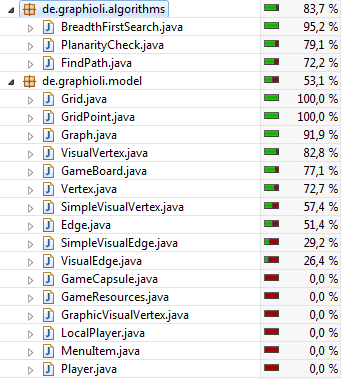
\includegraphics{code_coverage.png}
	\caption{Code coverage of the unit tests.}
	\label{img:codeCoverage}
\end{figure}
